% Source: AESP_466_ClassWork/Supplements/Notes/latex/6.2.4/6.2.4.tex

\documentclass[border=4pt]{standalone}
\usepackage{amsmath,amssymb,amsthm}
\usepackage{graphicx}
\usepackage{tikz}
\usepackage{xcolor}
\usetikzlibrary{arrows.meta,calc,positioning,decorations.markings,patterns,shapes.geometric,angles,quotes}

\definecolor{Garnet}{HTML}{73000A}
\definecolor{USC_Rose}{HTML}{CC2E40}
\definecolor{USC_Blue}{HTML}{466A9F}
\definecolor{USC_Slate}{HTML}{1F414D}
\definecolor{USC_Olive}{HTML}{65780B}
\definecolor{USC_Lime}{HTML}{CED318}
\definecolor{USC_Gold}{HTML}{A49137}
\definecolor{USC_Black90}{HTML}{565556}
\definecolor{USC_Black10}{HTML}{ECECEC}

\newcommand{\vect}[1]{\mathbf{#1}}
\newcommand{\mat}[1]{\mathbf{#1}}
\newcommand{\uvec}[1]{\hat{\mathbf{#1}}}
\newcommand{\transpose}{^{\mkern-1.5mu\mathsf{T}}}
\newcommand{\inv}{^{-1}}
\newcommand{\deriv}[2]{\frac{d #1}{d #2}}
\newcommand{\pderiv}[2]{\frac{\partial #1}{\partial #2}}

\begin{document}
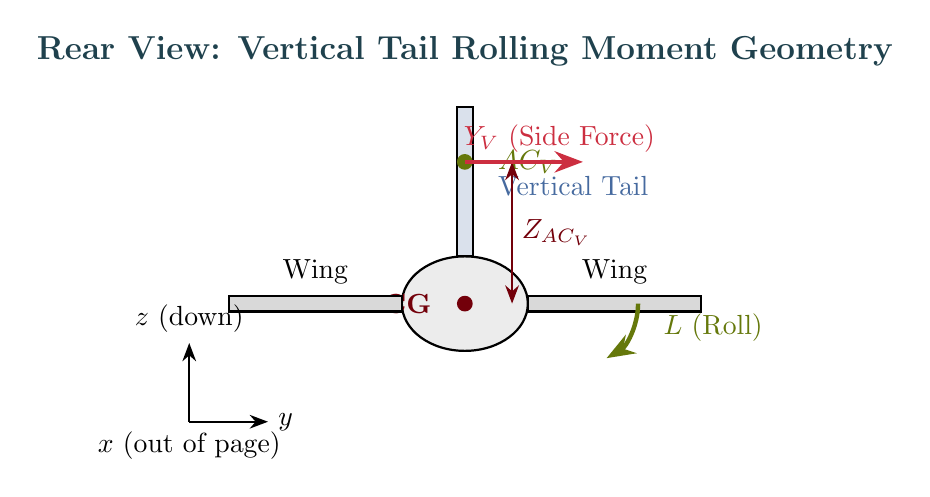
\begin{tikzpicture}[>=Stealth, scale=1.0]
    % Aircraft fuselage cross-section (rear view)
    \draw[thick, fill=USC_Black10] (0,0) ellipse (0.8 and 0.6);

    % CG marker
    \fill[Garnet] (0,0) circle (0.1);
    \node[Garnet, left] at (-0.3,0) {\textbf{CG}};

    % Vertical tail (simplified as rectangle)
    \draw[thick, fill=USC_Blue!20] (-0.1,0.6) rectangle (0.1,2.5);
    \node[USC_Blue, right] at (0.3,1.5) {Vertical Tail};

    % AC of vertical tail
    \fill[USC_Olive] (0,1.8) circle (0.1);
    \node[USC_Olive, right] at (0.3,1.8) {$AC_V$};

    % Moment arm Z_AC_V
    \draw[<->, thick, Garnet] (0.6,0) -- (0.6,1.8);
    \node[Garnet, right] at (0.6,0.9) {$Z_{AC_V}$};

    % Wing stubs (for reference)
    \draw[thick, fill=gray!30] (-3,-0.1) rectangle (-0.8,0.1);
    \draw[thick, fill=gray!30] (0.8,-0.1) rectangle (3,0.1);
    \node at (-1.9,0.4) {Wing};
    \node at (1.9,0.4) {Wing};

    % Side force arrow
    \draw[->, ultra thick, USC_Rose] (0,1.8) -- (1.5,1.8);
    \node[USC_Rose, above] at (1.2,1.8) {$Y_V$ (Side Force)};

    % Rolling moment arrow (curved)
    \draw[->, ultra thick, USC_Olive] (2.2,0) arc (0:-60:0.8);
    \node[USC_Olive, right] at (2.4,-0.3) {$L$ (Roll)};

    % Coordinate axes
    \draw[->, thick] (-3.5,-1.5) -- (-2.5,-1.5) node[right] {$y$};
    \draw[->, thick] (-3.5,-1.5) -- (-3.5,-0.5) node[above] {$z$ (down)};
    \node at (-3.5,-1.8) {$x$ (out of page)};

    % Title
    \node[font=\large\bfseries, USC_Slate] at (0,3.2) {Rear View: Vertical Tail Rolling Moment Geometry};

\end{tikzpicture}
\end{document}
